%%This is a very basic article template.
%%There is just one section and two subsections.
\documentclass[english,a4paper]{scrartcl}

\usepackage{graphicx}
\usepackage{listings}
\usepackage{color}
\usepackage{makeidx}
\usepackage{hyperref}
\usepackage{parskip}
\usepackage{multirow}
\usepackage{tocloft}
\renewcommand{\cftsecaftersnumb}{\hspace{6em}}
\renewcommand{\cftsubsecaftersnumb}{\hspace{6em}}
\renewcommand{\cftsubsubsecaftersnumb}{\hspace{6em}}

\makeindex

\hypersetup{
    %bookmarks=true,         % show bookmarks bar?
    unicode=false,          % non-Latin characters in Acrobat’s bookmarks
    pdftoolbar=true,        % show Acrobat’s toolbar?
    pdfmenubar=true,        % show Acrobat’s menu?
    pdffitwindow=false,     % window fit to page when opened
    pdfstartview={FitH},    % fits the width of the page to the window
    pdftitle={TDT4205 Compilers - Exercise 5 - hvatum},    % title
    pdfauthor={Stian Hvatum},     % author
    pdfsubject={TDT4205 Compilers},   % subject of the document
    pdfcreator={Stian Hvatum},   % creator of the document
    pdfproducer={Stian Hvatum}, % producer of the document
    pdfnewwindow=true,      % links in new window
    colorlinks,       % false: boxed links; true: colored links
    linkcolor=black,          % color of internal links
    citecolor=green,        % color of links to bibliography
    filecolor=magenta,      % color of file links
    urlcolor=cyan           % color of external links
}

\definecolor{listinggray}{gray}{0.9}
\definecolor{lbcolor}{rgb}{0.9,0.9,0.9}
\lstset{
    keywordstyle=\bfseries\ttfamily\color[rgb]{0,0,1},
    identifierstyle=\ttfamily,
    commentstyle=\color[rgb]{0.133,0.545,0.133},
    stringstyle=\ttfamily\color[rgb]{0.627,0.126,0.941},
    showstringspaces=false,
    basicstyle=\tiny,
    numberstyle=\tiny,
    framexleftmargin=3pt,
    numbers=left,
    stepnumber=1,
    numbersep=15pt,
    tabsize=2,
    breaklines=true,
    prebreak = \raisebox{0ex}[0ex][0ex]{\ensuremath{\hookleftarrow}},
    breakatwhitespace=false,
    aboveskip={1.5\baselineskip},
    columns=fixed,
    upquote=true,
    extendedchars=true,
  	frame=l,
    sensitive=true,
}
\lstdefinelanguage{vsl}
  {morekeywords={FUNC,VAR,PRINT},
  sensitive=false,
  morecomment=[l]{//},
  morecomment=[s]{/*}{*/},
  morestring=[b]",
}


\renewcommand{\thesection}{PART \arabic{section}}
\renewcommand{\thesubsection}{Task \arabic{section}.\arabic{subsection}}
\renewcommand{\thesubsubsection}{\arabic{subsubsection}.}

\title{TDT4205 Compilers\\
\Huge Exercise 5}
\author{Stian Hvatum (hvatum)\\MTDT}

\begin{document}
\maketitle
\tableofcontents
\newpage
\section{Theory}
\begin{minipage}[b]{0.5\linewidth}
 \centering
\subsection{Data flow analysis}
\subsubsection{Tree-address code}
\begin{lstlisting}[language=C,morekeywords={ifFalse}]
// for (int x=0; x<n; x++)
	x = -1
F1:	x = x + 1
	ifFalse x < n goto Nd

// for (int y=0; y<n-1; y++)	
	y = -1
F2:	y = y + 1
	m = n - 1
	ifFalse y < m goto F1
	
// if (array[y] > array[y+1]	
	y1 = y + 1
	ifFalse array[y] > array[y1] goto F2
// if-body
	y2 = y + 1
	temp = array[y2]
	y3 = y + 1
	array[y3] = array[y]
	array[y] = temp
// end of if, back to beginning of inner loop
	goto F2
Nd:	// end
\end{lstlisting}
 
 \end{minipage}
 \hspace{0.5cm}
 \begin{minipage}[b]{0.5\linewidth}
 \centering
\subsubsection{}
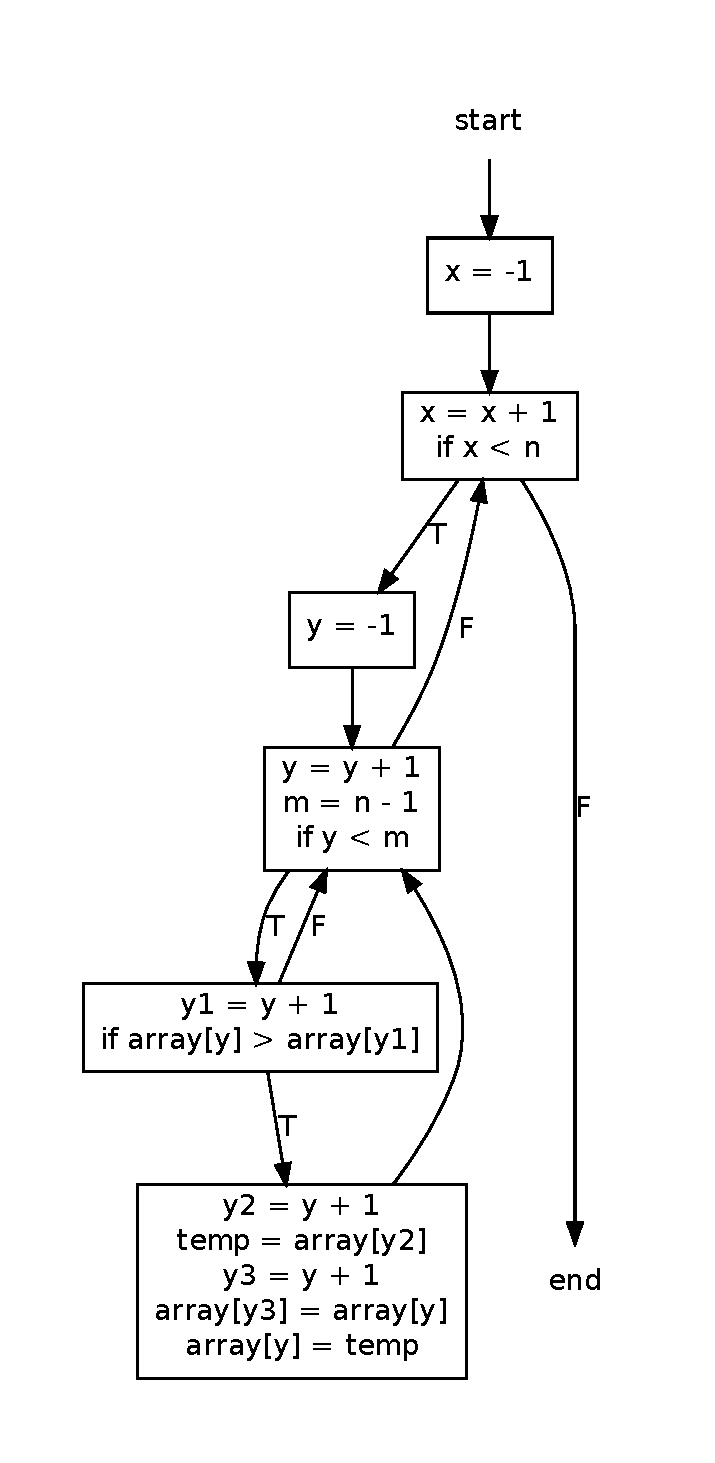
\includegraphics[height=250px]{flowgraph.pdf}

 \end{minipage}


 \begin{minipage}[b]{0.5\linewidth}
 \centering
\subsubsection{}
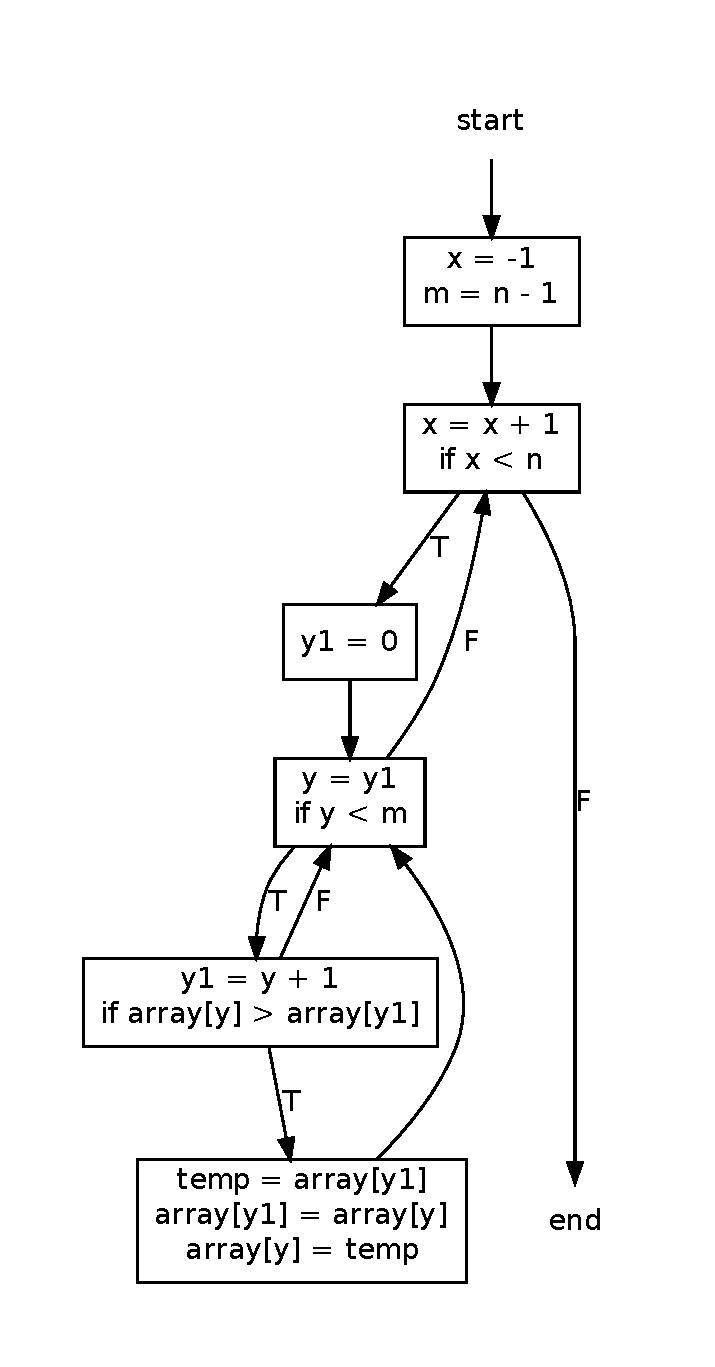
\includegraphics[height=300px]{flowgraph_optimized.pdf}
 \end{minipage}
  \hspace{0.5cm}
 \begin{minipage}[b]{0.5\linewidth}
 \centering
 \begin{itemize}
    \item
 Global and local common subexpression elimination
 \begin{enumerate}
   \item m = n - 1 is allways the same, but has been calculated once for each
   round in the loop. This is now put outside the loops.
 \end{enumerate}
    \item
    Copy propagation
    \begin{enumerate}
      \item y1, y2 and y3 share the same value, evaluate once.
      \item next y is allways the same as previous y1, no need to evaluate
      again.
    \end{enumerate}
   \item 
Constant folding
\begin{enumerate}
  \item No constants are given in the code in such a way that we can fold them.
\end{enumerate}
   \item 
 Dead code elimination
 \begin{enumerate}
   \item There is no longer any need for y2 and y3, so they are removed. 
 \end{enumerate}
 \end{itemize}
 \end{minipage}
 \newpage
\subsection{}
\subsubsection{Dominators}
A dominator is a node that is traversed on every possible path from the
\emph{start node} to node \emph{n}. This is important since if we know that a
node \emph{k} dominates an other node \emph{n}, \emph{k} has to be executed
before \emph{n} in every possible execution path, and thereby we can rely on its
content when considering node \emph{n}.

\subsubsection{Forward- and backwards analysis}
Forward- and backwards analysis have different objectives in terms of
optimization. During a forward analysis, we can calculate what statements may
have been encountered at each point, and make desisions of what paths a program
may and may not take.

During backwards analysis, we can calculate the \emph{liveness} of variables,
that is see wherever a variable is used after an  assignment. If a variable is
never read, or is never read after a certain point, is is ``dead'', and all
code relating to it after that point may be eliminated. Also called ``Dead code
elminination''.

\end{document}
